\documentclass[ignorenonframetext,]{beamer}
\usefonttheme{structurebold}
\setbeamertemplate{caption}[numbered]
\setbeamertemplate{caption label separator}{:}
\setbeamercolor{caption name}{fg=normal text.fg}
\usepackage{amssymb,amsmath}
\usepackage{ifxetex,ifluatex}
\usepackage{fixltx2e} % provides \textsubscript
\usepackage{lmodern}
\ifxetex
  \usepackage{fontspec,xltxtra,xunicode}
  \defaultfontfeatures{Mapping=tex-text,Scale=MatchLowercase}
  \newcommand{\euro}{€}
\else
  \ifluatex
    \usepackage{fontspec}
    \defaultfontfeatures{Mapping=tex-text,Scale=MatchLowercase}
    \newcommand{\euro}{€}
  \else
    \usepackage[T1]{fontenc}
    \usepackage[utf8]{inputenc}
      \fi
\fi
% use upquote if available, for straight quotes in verbatim environments
\IfFileExists{upquote.sty}{\usepackage{upquote}}{}
% use microtype if available
\IfFileExists{microtype.sty}{\usepackage{microtype}}{}

% Comment these out if you don't want a slide with just the
% part/section/subsection/subsubsection title:
\AtBeginPart{
  \let\insertpartnumber\relax
  \let\partname\relax
  \frame{\partpage}
}
\AtBeginSection{
  \let\insertsectionnumber\relax
  \let\sectionname\relax
  \frame{\sectionpage}
}
\AtBeginSubsection{
  \let\insertsubsectionnumber\relax
  \let\subsectionname\relax
  \frame{\subsectionpage}
}

\setlength{\parindent}{0pt}
\setlength{\parskip}{6pt plus 2pt minus 1pt}
\setlength{\emergencystretch}{3em}  % prevent overfull lines
\setcounter{secnumdepth}{0}
\definecolor{Black1}{RGB}{43,40,40}
\definecolor{Blue1}{RGB}{48, 122, 190}
\definecolor{Blue2}{RGB}{99, 151, 205}
\definecolor{Orange1}{HTML}{F5996F}
\definecolor{White1}{RGB}{255,255,243}
\definecolor{Grey1}{RGB}{164, 173, 185}
\definecolor{Grey2}{RGB}{244, 244, 244}
\usepackage{zxjatype}
\setjamainfont{Hiragino Kaku Gothic Pro}
\setbeamertemplate{navigation symbols}{}
\setbeamertemplate{itemize item}{\textcolor{Blue2}{\faOk}}
\setbeamertemplate{itemize subitem}{\textcolor{Black1}{\faThumbsDown}}
\hypersetup{colorlinks = true, linkcolor = blue, citecolor = red, urlcolor = Black1}
\usepackage{fontspec}
\usepackage{fontawesome}
\usepackage{scrextend}
\changefontsizes{17pt}
\usepackage{nruby}
\usepackage{ulem}
\usepackage{soul}
\setulcolor{magenta}
\setstcolor{Black1}
\sethlcolor{Grey2}
\setbeamerfont{title}{size = \fontsize{38}{10}}
\setbeamercolor{title}{fg = Blue1}
\setbeamerfont{subtitle}{size = \Large}
\setbeamercolor{subtitle}{fg = Blue2}
\setbeamercolor{author}{fg = Black1}
\setbeamercolor{normal text}{fg = Black1}
\setbeamerfont{date}{series = \itshape}
\setbeamercolor{date}{fg = Grey1}
\setbeamercolor{frametitle}{fg = Blue1}
\setbeamerfont{frametitle}{size = \Large}
\setbeamerfont{footnote}{size = \tiny}
\setbeamercolor{enumerate item}{fg = Blue2}

\title{前処理のための前処理}
\subtitle{シリーズ前処理2015}
\author{@u\_ribo}
\date{Tokyo.R\#45 January 17, 2015}

\begin{document}
\frame{\titlepage}

\begin{frame}

\center{
  \Huge{\textbf{\textcolor{magenta}{Tokyo.R} \\シリーズ前処理: \\おさらい}}
}

\end{frame}

\begin{frame}{\faFood 前処理}

\center{
  \large{【広義】手元にある観測データを、\\意図する分析手法が適用できる形にまで\\もっていく方法}
}

\begin{quote}
\scriptsize{\faLink http://www.slideshare.net/dichika/maeshori-missing}
\end{quote}

\end{frame}

\begin{frame}{\faTime 解析時間のほとんどは前処理}

\includegraphics{images/work_time_ratio-1.pdf}

\flushright{\scriptsize{\faBook Dasu and Johnson 2003.\\ Exploratory Data Mining and Data Cleaning. \textit{Wiley}}}

\end{frame}

\begin{frame}

{[}1{]} ``無駄'' ``無駄'' ``無駄'' ``無駄'' ``無駄'' ``無駄'' ``無駄''
``無駄'' {[}9{]} ``無駄'' ``無駄'' ``無駄'' ``無駄'' ``無駄'' ``無駄''
``無駄'' ``無駄'' {[}17{]} ``無駄'' ``無駄'' ``無駄'' ``無駄'' ``無駄''
``無駄'' ``無駄'' ``無駄'' {[}25{]} ``無駄'' ``無駄'' ``無駄'' ``無駄''
``無駄'' ``無駄'' ``無駄'' ``無駄'' {[}33{]} ``無駄'' ``無駄'' ``無駄''
``無駄'' ``無駄'' ``無駄'' ``無駄'' ``無駄'' {[}41{]} ``無駄'' ``無駄''
``無駄'' ``無駄'' ``無駄'' ``無駄'' ``無駄'' ``無駄'' {[}49{]} ``無駄''
``無駄'' ``無駄'' ``無駄'' ``無駄'' ``無駄'' ``無駄'' ``無駄'' {[}57{]}
``無駄'' ``無駄'' ``無駄'' ``無駄'' ``無駄'' ``無駄'' ``無駄'' ``無駄''
{[}65{]} ``無駄'' ``無駄'' ``無駄'' ``無駄'' ``無駄'' ``無駄'' ``無駄''
``無駄'' {[}73{]} ``無駄'' ``無駄'' ``無駄'' ``無駄'' ``無駄'' ``無駄''
``無駄'' ``無駄''

\end{frame}

\begin{frame}

\center{
  \large{前処理に時間がかかる \\-> 最終的な出力結果の質が低下する}\\\vspace{0.6em}
  \fontsize{120}{10}{\faThumbsDown \faThumbsDown \faThumbsDown}
}

\end{frame}

\begin{frame}

{[}1{]} ``どうしてこうなった'' ``どうしてこうなった'' {[}3{]}
``どうしてこうなった'' ``どうしてこうなった'' {[}5{]}
``どうしてこうなった'' ``どうしてこうなった'' {[}7{]}
``どうしてこうなった'' ``どうしてこうなった'' {[}9{]}
``どうしてこうなった'' ``どうしてこうなった'' {[}11{]}
``どうしてこうなった'' ``どうしてこうなった'' {[}13{]}
``どうしてこうなった'' ``どうしてこうなった'' {[}15{]}
``どうしてこうなった'' ``どうしてこうなった'' {[}17{]}
``どうしてこうなった'' ``どうしてこうなった'' {[}19{]}
``どうしてこうなった'' ``どうしてこうなった'' {[}21{]}
``どうしてこうなった'' ``どうしてこうなった'' {[}23{]}
``どうしてこうなった'' ``どうしてこうなった'' {[}25{]}
``どうしてこうなった'' ``どうしてこうなった'' {[}27{]}
``どうしてこうなった'' ``どうしてこうなった'' {[}29{]}
``どうしてこうなった'' ``どうしてこうなった''

\end{frame}

\begin{frame}

\center{
  \large{\textcolor{magenta}{Tokyo.R} シリーズ前処理}\\
  \Huge{\textbf{今日のテーマ: \\\textcolor{Blue1}{前}処理のための\\\textcolor{magenta}{前}処理}}
}

\end{frame}

\begin{frame}{\large{もちべーしょん: 前処理の苦労を減らしたい}}

内容\ldots{}

\begin{itemize}
\itemsep1pt\parskip0pt\parsep0pt
\item
  データ解析、前処理における\textbf{環境構築、心がけ}
\item
  ぼくのがんがえたこうりつてきなまえしょり、\textbf{そのためにひつようなまえしょり}
\end{itemize}

\large{\faHandLeft 議論を通じて知識・理解を深めたい}

\end{frame}

\begin{frame}

\center{
  \Huge{\textbf{\textit{\textcolor{magenta}{\#Tsurami}}}}
}

\end{frame}

\begin{frame}{\textit{\textcolor{magenta}{\#Tsurami}}}

\center{
  
\includegraphics{images/tsurami.png}
  
  \textit{\scriptsize{\faTwitter https://twitter.com/yamano357/status/552514988137783301}}
}

\end{frame}

\begin{frame}{\textit{\textcolor{magenta}{\#Tsurami}}}

\center{
  
\includegraphics{images/tsurami2.png}
  
  \textit{\scriptsize{\faTwitter https://twitter.com/gg$\_$hatano/status/551328451068588032}}
}

\end{frame}

\begin{frame}{\textit{\textcolor{magenta}{\#Tsurami}}}

\center{
  Japan.R2014 \textcolor{magenta}{所\ruby{沢}{さわ}}さんの\href{http://www.slideshare.net/TokorosawaYoshio/japanr2014}{発表\faExternalLink}より...

  Remember \faQuoteLeft \textcolor{Blue2}{why are you using SJIS?} \faQuoteRight

  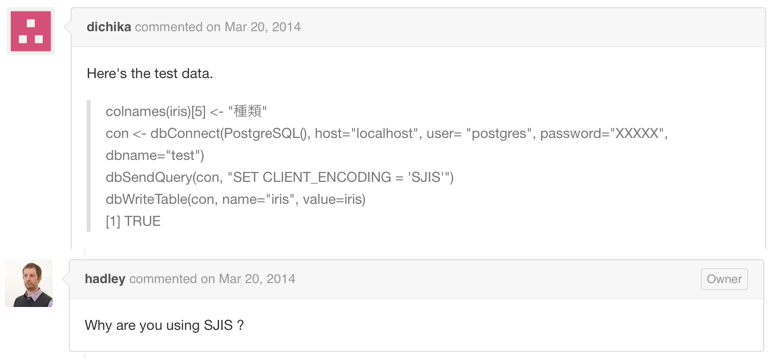
\includegraphics{images/why_are_u_using_sjis.png}

  \textit{\scriptsize{\faGithub https://github.com/hadley/dplyr/issues/339}}
}

\end{frame}

\begin{frame}{\faThumbsDown 前処理を行う際に生じる問題の原因}

\begin{itemize}
\itemsep1pt\parskip0pt\parsep0pt
\item
  Are you okay?

  \begin{itemize}
  \itemsep1pt\parskip0pt\parsep0pt
  \item
    邪智暴虐な俺々ファイルの存在
  \item
    コメントのない奇怪なコード
  \item
    作業過程の再現性の欠如
  \item
    とりあえず、的に書かれたコード
  \end{itemize}
\end{itemize}

\end{frame}

\begin{frame}

{[}1{]} ``滅'' ``滅'' ``滅'' ``滅'' ``滅'' ``滅'' ``滅'' ``滅'' ``滅''
``滅'' ``滅'' {[}12{]} ``滅'' ``滅'' ``滅'' ``滅'' ``滅'' ``滅'' ``滅''
``滅'' ``滅'' ``滅'' ``滅'' {[}23{]} ``滅'' ``滅'' ``滅'' ``滅'' ``滅''
``滅'' ``滅'' ``滅'' ``滅'' ``滅'' ``滅'' {[}34{]} ``滅'' ``滅'' ``滅''
``滅'' ``滅'' ``滅'' ``滅'' ``滅'' ``滅'' ``滅'' ``滅'' {[}45{]} ``滅''
``滅'' ``滅'' ``滅'' ``滅'' ``滅'' ``滅'' ``滅'' ``滅'' ``滅'' ``滅''
{[}56{]} ``滅'' ``滅'' ``滅'' ``滅'' ``滅'' ``滅'' ``滅'' ``滅'' ``滅''
``滅'' ``滅'' {[}67{]} ``滅'' ``滅'' ``滅'' ``滅'' ``滅'' ``滅'' ``滅''
``滅'' ``滅'' ``滅'' ``滅'' {[}78{]} ``滅'' ``滅'' ``滅'' ``滅'' ``滅''
``滅'' ``滅'' ``滅'' ``滅'' ``滅'' ``滅'' {[}89{]} ``滅'' ``滅'' ``滅''
``滅'' ``滅'' ``滅'' ``滅'' ``滅'' ``滅'' ``滅'' ``滅'' {[}100{]} ``滅''
``滅'' ``滅'' ``滅'' ``滅'' ``滅'' ``滅'' ``滅'' ``滅'' ``滅'' ``滅''

\end{frame}

\begin{frame}{\faBullhorn Rを使った\textcolor{magenta}{前処理5原則}}

\begin{enumerate}
\def\labelenumi{\arabic{enumi}.}
\itemsep1pt\parskip0pt\parsep0pt
\item
  作業はRStudio内ですべて完結させる
\item
  \hl{.Rproj}を作成する
\item
  \hl{.Rmd}でファイルを保存する
\item
  Gitによるバージョン管理をおこなう
\item
  プロジェクトのガイドラインを策定する
\end{enumerate}

\end{frame}

\begin{frame}{Rにおける統合開発環境: RStudio}

\begin{columns}[T]
  \begin{column}[T]{6cm}
    \begin{itemize}
      \item そろそろ ver.0.99
      \item Viewerの強化
      \item パッケージ名の補完
      \item \scriptsize{ref) \faLink http://goo.gl/inFdt5}
    \end{itemize}
  \end{column}
  \begin{column}[T]{4cm}
    
\includegraphics[scale = 0.25]{images/webshot_rstudio_com.png}
  \end{column}
\end{columns}

\large{\faHandLeft これから説明する内容は\\すべてRStudio上で行える}

\end{frame}

\begin{frame}

\center{
  \Huge{\faCoffee 話題閑話}
}

\end{frame}

\begin{frame}

\center{
  \Huge{\textbf{絶許}}
  
  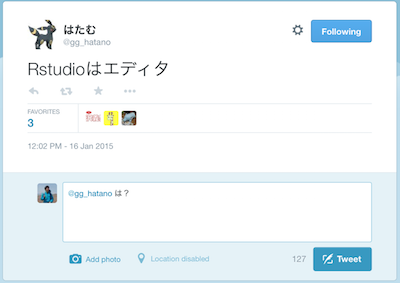
\includegraphics{images/gg_hatamu_tweet.png}
  
  \textit{\scriptsize{\faTwitter https://twitter.com/gg$\_$hatano/status/555923067675738113}}
}

\end{frame}

\begin{frame}{.Rproj}

\begin{itemize}
\itemsep1pt\parskip0pt\parsep0pt
\item
  フォルダ内にフォルダ名.Rprojというファイルが生成
\item
  RStudioの設定などが記述される
\end{itemize}

\begin{block}{ご利益}

\begin{itemize}
\itemsep1pt\parskip0pt\parsep0pt
\item
  面倒なフォルダ指定、\hl{setwd}からの開放
\item
  パッケージ管理ツール Packratの利用
\item
  Gitの運用
\end{itemize}

\end{block}

\end{frame}

\begin{frame}

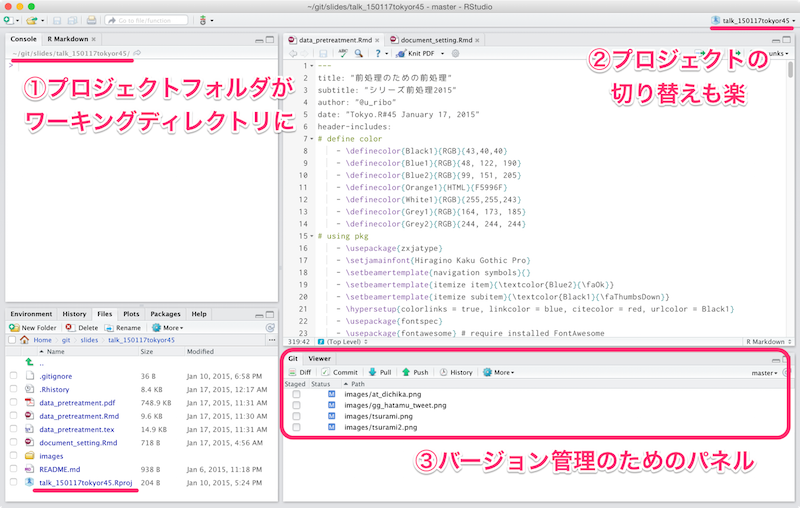
\includegraphics[scale = 0.8]{images/rstudio_panel.png}

\end{frame}

\begin{frame}{.Rmd: R + Markdown + \LaTeX}

\center{
  \Huge{= \textcolor{magenta}{POWERFUL} \faRocket}
  
  \normalsize{このスライドも\hl{.Rmd}で書いている
  
  \faGithub \href{https://github.com/uribo/lab.note}{\hl{lab.note}}パッケージでどうぞ \footnote{ただしWindows、Linux、テメーらはダメだ(\textcolor{magenta}{未検証})}
  
  \tiny{\hl{rmarkdown::draft("MyReport.Rmd",template="basic$\_$report",package="lab.note")}
  }}
}

\end{frame}

\begin{frame}{アウトプットオオオオオオオオ!!!!}

ぼく「(モニターで確認して)よし、これでいいな」

ボス「図を印刷して見せて」

ぼく「(あああああああああ!!!!!!!!!)」

\flushright{\faHandLeft \LaTeX おじさんが誕生した \footnote{HTMLでの出力はモニター向け。PDFを印刷したいよね、と。\textit{Word? しらん}}}

\end{frame}

\begin{frame}{Git: 分散型バージョン管理システム}

\begin{itemize}
\itemsep1pt\parskip0pt\parsep0pt
\item
  長い時間を経てプロジェクトは完成される
\item
  完成後も管理し続ける必要が生じる
\item
  同様の処理を、別プロジェクトで、自分以外の誰かが行う場合がある
\end{itemize}

\faHandLeft 記録として残すことが大事

\end{frame}

\begin{frame}{GitHubで広がるコミュニケーション}

\begin{itemize}
\itemsep1pt\parskip0pt\parsep0pt
\item
  パッケージを作って公開
\item
  今日からあなたも開発者
\item
  芝を生やしてもちべーしょんを高めよう!
\end{itemize}

\center{
  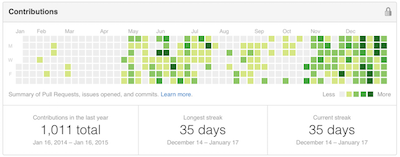
\includegraphics{images/contribution.png}
}

\end{frame}

\begin{frame}{README $\fallingdotseq$ 嫁}

\begin{itemize}
\itemsep1pt\parskip0pt\parsep0pt
\item
  リポジトリ(プロジェクト)の顔
\item
  迷った際はここを見れば解決できるように

  \begin{enumerate}
  \def\labelenumi{\arabic{enumi}.}
  \itemsep1pt\parskip0pt\parsep0pt
  \item
    作業のワークフローを書く
  \item
    ファイル名、関数名の規則
  \item
    プロットの色、サイズ
  \end{enumerate}
\end{itemize}

\end{frame}

\begin{frame}{\faMagic Tips}

\begin{itemize}
\itemsep1pt\parskip0pt\parsep0pt
\item
  とにかく日本語はNG

  \begin{itemize}
  \itemsep1pt\parskip0pt\parsep0pt
  \item
    SJIS
  \end{itemize}
\item
  犬 -\textgreater{} \hl{INU}にするなら辞書をひいて\hl{dog}に

  \begin{itemize}
  \itemsep1pt\parskip0pt\parsep0pt
  \item
    ローマ字カナも良くない
  \end{itemize}
\item
  Excelは入力・閲覧用 -\textgreater{} \hl{dplyr}パッケージで

  \begin{itemize}
  \itemsep1pt\parskip0pt\parsep0pt
  \item
    単位変換、新たな列の作成は闇
  \end{itemize}
\item
  ハイフン、アンダーバーをどう扱うか

  \begin{itemize}
  \itemsep1pt\parskip0pt\parsep0pt
  \item
    スペースの落とし穴 (\LaTeX)
  \end{itemize}
\end{itemize}

\end{frame}

\begin{frame}

\center{
  \Huge{「いろいろと\textcolor{Blue2}{面倒}だ」}  
}

\end{frame}

\begin{frame}

\center{    
  \LARGE{「でも、あなたのちっぽけな\\\textbf{\textcolor{magenta}{頭では忘れてしまう}}\\でしょう(煽り)」}\
    
  \footnotesize{「ぐぬぬ」}
}

\end{frame}

\begin{frame}

\center{
  \Huge{\textbf{\textcolor{magenta}{\faUser 自分のため、\\\faGroup 仲間のため、\\\faGlobe 誰かのため}}}
}

\flushright{\textit{Let's go! \faRocket}}

\end{frame}

\begin{frame}{@dichika進捗どうですか\faEyeOpen}

\center{
  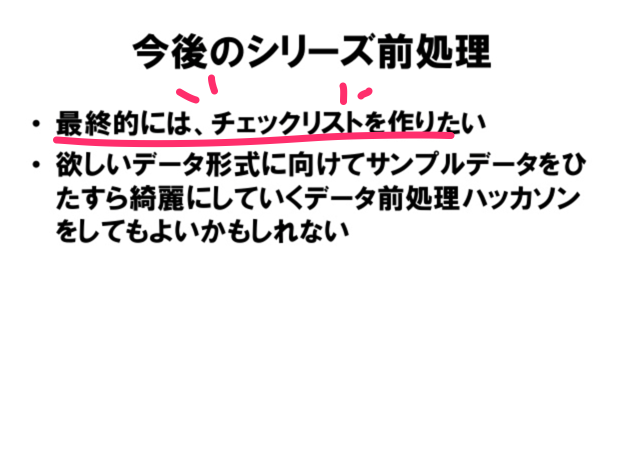
\includegraphics[angle = -3]{images/at_dichika.png}
  
  \textit{\scriptsize{\faLink http://www.slideshare.net/dichika/maeshori-missing}}
}

\end{frame}

\begin{frame}{\Large{みんなで \textit{\textcolor{magenta}{\#Tsurami}} を供養しよう}}

\center{
  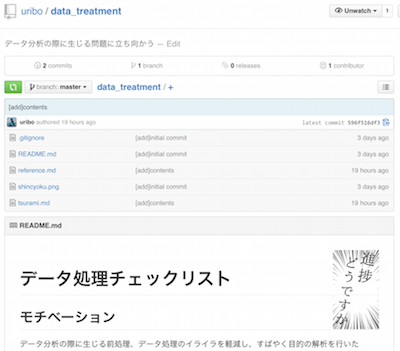
\includegraphics[scale = 0.25]{images/github_uribo_data_treatment.png}
  
  \textit{\scriptsize{\faGithub https://github.com/uribo/data$\_$treatment}}
}

\end{frame}

\begin{frame}{\small{Sessioninfo: R version 3.1.2 (2014-10-31)}}

{[}1{]} ``webshot'' ``ggthemr'' ``knitcitations'' {[}4{]} ``fortunes''
``xtable'' ``rmarkdown''\\ {[}7{]} ``devtools'' ``popbio''
``quadprog''\\{[}10{]} ``ggplot2'' ``glmmML'' ``dplyr''\\{[}13{]}
``magrittr'' ``MASS'' ``lattice''\\{[}16{]} ``stringr'' ``knitr''

\flushright{\textit{\textcolor{magenta}{Questions?}} \faComments}

\end{frame}

\end{document}
